%%%%% Document Setup %%%%%%%%

\documentclass[10pt,twocolumn]{revtex4}    % Font size (10,11 or 12pt) and column number (one or two).

\usepackage{times}                          % Times New Roman font type

\usepackage{array}

\usepackage[a4paper, left=1.85cm, right=1.85cm,top=1.85cm, bottom=1.85cm]{geometry}       % Defines paper size and margin length

\usepackage[font=small, labelfont=bf]{caption}                      % Defines caption font size as 9pt and caption title bolded
\newcommand{\mycomment}[1]{}

\usepackage[sorting=none]{biblatex}
\addbibresource{refs.bib}


\usepackage{graphics,graphicx,epsfig,ulem}	% Makes sure all graphics works
\usepackage{amsmath} 						% Adds mathematical features for equations

\usepackage{etoolbox}                       % Customise date to preferred format

\makeatletter
\patchcmd{\frontmatter@RRAP@format}{(}{}{}{}
\patchcmd{\frontmatter@RRAP@format}{)}{}{}{}
\renewcommand\Dated@name{}
\makeatother

\usepackage{fancyhdr}


\pagestyle{fancy}                           % Insert header
\renewcommand{\headrulewidth}{0pt}
\lhead{J. K. Read}                          % Your name
\rhead{A Charminingly Simple Method for Predicting Quarkonium Mass}            % Your report title               

\def\bibsection{\section*{References}}        % Position reference section correctly


%%%%% Document %%%%%    
\begin{document}


\title{A Charminingly Simple Method for Predicting Quarkonium Mass} 
\date{Submitted: \today{}, Experimental Period: October 20, 2022 - March 25, 2023}
\author{J. K. Read}
\affiliation{\normalfont L3 Computing Project, Lab Group: C4, Lab Day: Thursday 11pm}


\begin{abstract}              
 
Quarkonium is a bound state of a heavy quark and its antiquark, charm quarks making charmonium and bottom quarks making bottomonium. These quarkonia can be described by Schr\"odinger's equation and have its properties analysed just like any other quantum mechanical system. This includes its binding energy eigenvalue, when can be found numerically by solving a pair of coupled ODEs derived from Schr\"odinger's at some lower bound of the eigenvalue, and increasing this value until the correct wavefunction behaviour is exhibited. Then the eigenvalue is added to the mass of the constituent quark masses to reproduce the mass of states up to 2S with good agreement using a number of models for the inter quark potential, $M_{\eta_c(1S)} = 2.984GeV, M_{h_c(1P)} = 3.462GeV, M_{\eta_c'(2S)} = 3.675GeV$. Due to good agreement with experimental masses, masses of unmeasured states can be predicted with a sense of validity, $M_{h_c'(2P)} = 4.003GeV, M_{\eta_c''(3S)} = 4.190GeV$. This method works well, reproducing masses with good agreement, for one parameter potential models, however struggles with multi-parameter models due to time complexity, and is also sensitive to numerical instability due to small numbers in computer memory. 

\end{abstract}

\maketitle

\thispagestyle{plain} % produces page number for front page

\section{Introduction} \label{sec:Introduction}
\subsection{Quarkonium as a Particle}\label{ssec:CharmoinumParticl}
Quarks are fundamental particles, three bound together by the strong force make up protons and neutrons. They can also be found in quark-antiquark pairs, again bound by the string force, called "Mesons". 
Because of technological advancement in high energy infrastructure in the 1970s, heavier particles were able to be created in accelerators at facilities such as BNL and SLAC. This lead to the joint discovery of the $J$ and $\psi$ particles by BNL and SLAC respectivly in 1974\textbf{\cite{BNLPaper}, \cite{SLACPaper}}, who after review agreed that these new particles were one in the same, and also, more importantly, that the new $J\psi$ particle must be made of a new charm, $c$, quark and its antiparticle, $\overline{c}$. The mass of this new quark was found to be $m_c = 0.27\pm0.02GeV$. This event started the so called November revolution \textbf{\cite{DiscoveryQuarks}}.
Later in 1977 the bottom, $b$, quark with mass $m_b = 4.18^{+0.03}_{-0.02}$\textbf{\cite{pdg}} was discovered at Fermilab\textbf{\cite{BottomPaper}}.
Mesons made of a heavier quarks and its own antiquark are given the name "Quarkonium"\textbf{\cite{PotentialModels}}. Charmonium is bound $c\overline{c}$ paris, with ground triplet state $J/\psi$, and bottomonium id bound $b\overline{b}$ pairs, with ground triplet state $\Upsilon$.


Like any quantum mechanical object, the charmonium state is characterised by $n$,$l$,$m$, the principle, azimuthal, and magnetic quantum numbers respectively; with each singlet state assigned a name: $\eta_c{1S}; h_c{1P}; \eta_c'{2S}; h_c'{2P}; \eta_c''{3S}$. The higher states (2P and above) have quarks with very high energy so the binding energy needed to hold them together must also be very high. Due to this, these particles are very unstable and so as yet do not have confirmed masses (though there is ongoing work into this, see \textbf{\cite{Kher_2019}}).


Therefore then, the aim of this work will be to use the ground state singlet state ($\eta_c{1S}$) to calibrate a method of predicting the mass of charmonium states, via solving Schr\"odinger's equation numerically. Then after calibration the masses of stable states will be predicted and compared to experimental masses of singlet states to ascertain the quality of agreement and validity of future results. Finally, if good agreement with experiment is found, predictions will be made of masses for states $h_c'{2P}$ and $\eta_c''{3S}$. 


 \subsection{Quantum Mechanical Basis}\label{ssec:QMBasis}
Despite being discovered due to high energy experiments, these heavy mesons can be described theoretically by non-relativistic quantum mechanics, because they have a small quark velocity, $v$ to speed of light, $c$, ratio ($\langle v^2/c^2\rangle _{J/\Psi} = 0.23$, $\langle v^2/c^2\rangle _{\Upsilon} = 0.08$) \textbf{\cite{PotentialModels}}.

Also, due to the symmetry of a $q\overline{q}$ pair the interaction potential, $V(r)$ between the quarks will be spherically symmetric. As well, non-potential effect (e.g. spin) will be small\textbf{\cite{PotentialModels}}. Therefore we can write the wavefunction, $\psi(r,\theta,\phi)_{n\ell m}$, of our heavy mesons as,

\begin{equation} \label{eqn:SpinlessWfn}
-\frac{\hbar}{2\mu}\nabla^2\psi_{n\ell m} + [V(r)-E_{n\ell}]\psi_{n\ell m} = 0, 
\end{equation}

via neglecting spin, where $\mu = (m_q+m_{\overline{q}})/(m_qm_{\overline{q}})$ is the reduced mass, r is the radial distance between the quarks, and $E_{n\ell}$ is the binding energy eigenvalue of $\psi_{n\ell m}$. 
As the system is spherically symmetric, $\psi(r,\theta,\phi)_{n\ell m}$ can be represented as the product of a radial component, $R_{n\ell}$, and a spherical harmonic, $Y_{\ell m}$,
\begin{equation}\label{eqn:splitWavefunction}
    \psi(r,\theta,\phi)_{n\ell m} = R_{n\ell}(r)Y_{\ell m}(\theta,\phi),
\end{equation}
such $u_{n \ell}(r) = rR_{n\ell}(r)$ satisfies
\begin{equation}\label{eqn:secondOrderODE}
    \frac{d^2 u_{r \ell}}{dr^2} - \frac{\ell(\ell + 1)}{r^2}u_{n \ell} + 2\mu(E_{n \ell} - V(r))u_{n \ell} = 0.
\end{equation}

These wavefunctions will be normalised such,
\begin{equation}\label{Normalisation}
    \int_{0}^{\infty} r^2|R_{n \ell}|^2 dr =  \int_{0}^{\infty} |u_{n \ell}|^2 dr = 1.
\end{equation}

After finding the binding energy of the $q\overline{q}$ pair, the mass of the meson for the given quantum numbers, $M_{n \ell}$, is
\begin{equation}\label{eqn:mesonMass}
    M_{n\ell} = m_q + m_{\overline{q}} + E_{n \ell},
\end{equation}
Where mass is measure in $GeV$, (natural units $\hbar=c=1$

\subsection{Potential Models}\label{ssec:PotModels}

\begin{figure}[t]
    \centering
    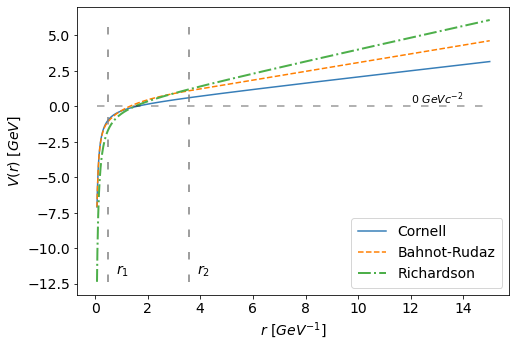
\includegraphics[width=\linewidth]{PotPlot.png}
    \caption{A plot of the Cornell \textbf{Eq.\ref{eqn:CornellV}}, Bhanot-Rudaz \textbf{Eq.\ref{eqn:BaRuV}}, and Richardson \textbf{Eq.\ref{eqn:RichV}} potentials $V(r)$ against $r$ with parameters $\beta_C \simeq 0.213$, $\beta_{BR} \simeq 0.206$, $\beta_R \simeq 0.410$. A gray dashed line is added to show the position of $V(r) = 0GeV$.}
    \label{fig:potPlot}
\end{figure}

Since the November Revolution started, by the discovery of the charm quark in 1974 \textbf{\cite{DiscoveryQuarks}}, there have been many models formulated to describe the potential between quark-antiquark pairs.
In the Cornell potential model \textbf{\cite{CornellPaper}}, the potential between the quarks in the meson can be parameterised in terms of the strong coupling constant,$\alpha_s$ and a chromodynamic tension, $\beta_{C}$,
\begin{equation}\label{eqn:CornellV}
    V_{C} = - \frac{4\alpha_s}{3r} + \beta_{C}r,
\end{equation}.

where $\alpha_s = 0.4$ between charm quarks, and is unitless in natural units. The first term is called a "coulombic" part due to its resemblance to the Coulomb potential, and is dominant at short ranges and represents one-gluon interactions \textbf{\cite{ColoumbonicValidPaper}}. The second part is a linear binding that describes the increase in strong force at large $r$. Both these terms are needed to mimic quantum chromodynamics (QCD).

Next the Bhanot-Rudaz (BR) potential \textbf{\cite{BhRoPaper}} suggest there is a 3rd regime between the short-range coulombic $1/r$ part and the long-rage linear $r$ part, a logarithmic part, which have the following ranges,

\begin{subequations}\label{eqn:BaRuV}
    \begin{equation}\label{eqn:BaRuPot}
        \begin{split}
        V_{BR}(r) = & -\frac{4}{3}\frac{\alpha_s}{r}, r \leq r_1, \\
                    &= b\ln{\frac{r_0}{r}}, r_1 \leq r \leq r_2, \\
                    & = \beta_{BR} r, r \geq r_2,\\
        \end{split}
    \end{equation}
\end{subequations}

where,

\begin{equation*}
    r_0 = (\frac{4}{3}\alpha_s)^{\frac{1}{2}} \beta_{BR}^{-1/2}, \text{   (7b)}; r_1 = \frac{r_0}{e}, \text{   (7c)},
\end{equation*}

\begin{equation*}
    r_2 = er_0, \text{   (7d)}; b = \beta_{BR}r_2 , \text{   (7e)}
\end{equation*}

and $e \approx 2.718$ is Euler's number, and $\beta_{BR}$ serves the same as $\beta_{C}$, a binding constant. The logarithmic part was motivated by the work of Quigg and Rosner to  give mass splittings independent $m_q$, however Bhanot and Rudaz found integrating this into a model still having a coulombic and confining term made better predictions of charmonium masses. 


L. P. Fulcher adapted the potential model of Richardson to create what this work will call the Richardson-Fulcher (RF) potential model \textbf{\cite{RichardsonPaper}}, in order to account for short-range perturbative QCD effects. Richardson expressed $\alpha_s(q^2) \propto 1/ln(|q^2|/\Lambda^2)$ where $q$ is  momentum transfer and $\Lambda$ is the QCD scale parameter, leading to a potential model \textbf{\cite{donoghue}},

\begin{equation}
    V_R(r) = -\frac{(8\pi)^2}{27}\mathcal{F}\{[q^2\ln{(\frac{q^2}{\Lambda^2})}]^{-1}\}.
\end{equation}

However to solve the arising singularity issue as $q\rightarrow \Lambda$, the substitution of $|q^2|/\Lambda^2 \rightarrow 1+|q^2|/\Lambda^2$ is made. However this blurs the connection between $\Lambda$ and the QCD scaling parameter, so Moxhay and Rosner decided to treat $\Lambda$ as a parameter. From there through Fulcher added a linear term in terms of the string constant, $\beta_{RF}$, to agree more with experiment \textbf{\cite{RichardsonPaper}}. Thus,
\begin{equation}\label{eqn:RichV}
    V_{RF}(r) = \beta_{RF}r - \frac{8\pi}{(33-2n_f)r} + ... ,
\end{equation}

(the first two terms of the Fourier transform are leading so calculation will be approximated to this) where $n_f = 3$ is the degrees of freedom of meson quarks.

Finally, the Martin potential model \textbf{\cite{MartinPaper}} is expressed via 3 parameters,
\begin{equation}\label{eqn:MartinV}
    V_{M} = Br^\alpha - A,
\end{equation}
where $\alpha = 0.100$\textbf{\cite{MartinPaper}}. This is a purely phenomenological model, not motivated by QCD, where $\alpha$ and $B$ decide on the shape of the potential, and $A$ translates in $V(r)$ space.


\section{Numerical Solution} \label{sec:numericalSolution}


In the following description of the numerical solving, $\beta$ will refer to in general the parameters of the potential models.


In order to solve the wavefunction numerically, a range and boundaries are needed. Firstly, the states will be solved in a range $r \in [10^{-6}, 15]GeV^{-1}$ with step size $\Delta_r \simeq 0.015GeV^{-1}$, with the lower bound to avoid annihilation and dividing by $0$ in numerical calculations, and the upper to mitigate effects of numerical divergence. Then, as wavefunction is well behaved at r = 0, so $u_{nl}(0) = 0$, and also $du_{n \ell}(0)/dr = 1$. For an upper bound, as $r \rightarrow \infty$, $u_{r \ell}(r)$ $\rightarrow$ 0, $du_{n \ell}(0)/dr$ $\rightarrow$ 0. 

Then to solve the wavefuntion numerically the \textbf{odeint} function from the \textbf{scipy.integrate} module will be called to numerically integrate a pair of coupled first order differential equations derived from \textbf{Eq.\ref{eqn:secondOrderODE}},
\begin{subequations}\label{eqn:coupledODEs}

    \begin{equation}\label{seqn:duODE}
        \frac{du_{n \ell}}{dr} = v_{n \ell}
    \end{equation}
    
    \begin{equation}\label{seqn:dvODE}
       \frac{dv_{n \ell}}{dr} = \frac{\ell(\ell + 1)}{r^2}u_{n \ell} - 2\mu(E_{n \ell} - V(r))u_{n \ell}
    \end{equation}
    
\end{subequations}
to find $u_{n\ell}$.


\begin{figure}[t]
    \centering
    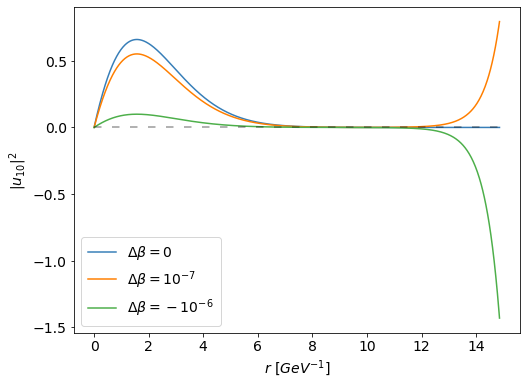
\includegraphics[width=\linewidth]{DivFlip.png}
    \caption{A plot of $|u_{10}|^2$ by $r$ using the cornell potential to demonstrate how a small change in the parameter value $\Delta \beta$ changes the behaviour of the divergence out toward $\sim15GeV^{-1}$.}
    \label{fig:divFlip}
\end{figure}

\begin{figure}
    \centering
    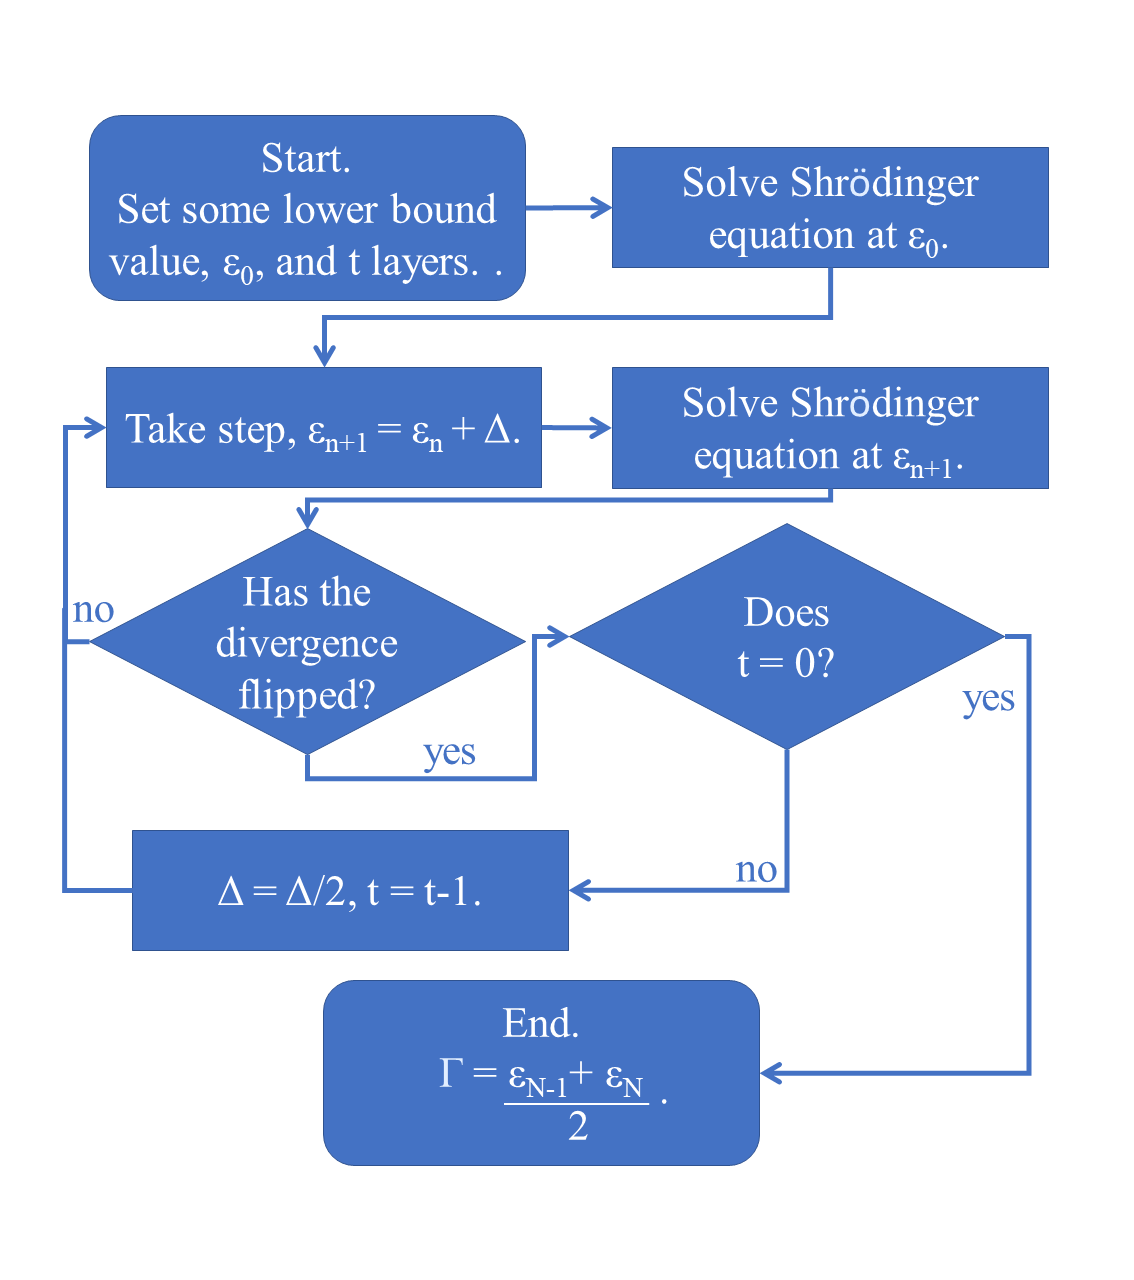
\includegraphics[width = \linewidth]{gammaflowchart.png}
    \caption{A flowchart showing the working of the step-method as described in \textbf{\ref{sec:numericalSolution}}.}
    \label{fig:flowchart}
\end{figure}

When the \textbf{Eq.\ref{eqn:coupledODEs}} set are computed using a $\beta$ or $E_{n\ell}$ that is different from the solution there will be a noticeable divergence positive or negative, which will flip as the solution is crossed and passed, seen in \textbf{Fig.\ref{fig:divFlip}}. Therefore, in stepping from some lower bound, $\epsilon_0$, of $\beta$ or $E_{n\ell}$, until a divergence flip at some $\epsilon_N$ a value can be found as,

\begin{equation}
    \Gamma = \frac{\epsilon_{N-1} + \epsilon_N}{2} = \epsilon_{N-1} + \frac{\Delta}{2}
\end{equation}

where $\Delta$ is the step size, and $\Gamma$ is $\beta$ or $E_{n\ell}$. 
The most accurate solution will be found where the divergence out at $r \sim 15GeV^{-1}$, what will be called the "tail," is minimal. In order to increase the accuracy of this process this method also applies what will be called layering to approach a tail of near $0$. The divergence flip signifies the solution is in-between the values of $\epsilon_{N-1}$ and $\epsilon_N$, however it may not be the mean of the two. So, to further approach the solution $\Delta$ is reduced by some factor and this new step size is then used to step from  $\epsilon_{N-1}$ again. This work has layered by halving $\Delta$ as finding which half of the range from $\epsilon_{N-1}$ to $\epsilon_N$ the solution is in will approach the solution the fastest. This layering can be repeated an arbitrary number of times in order to approach the solution to an arbitrary level of accuracy by reducing the tail closer to $0$ in each layer. A flowchart showing the entire process is seen in \textbf{Fig.\ref{fig:flowchart}}. 

To set which state is to be solved conditions of behaviour are needed in examination of the calculated wavefunction. The wavefunction will have a number of nodes, $N_0$, and turning points, $N_t$. These two properties should meet the conditions of $N_0 = n-1$ and $N_t = n$. This is strictly only true for $\ell = 0$, however for good agreement with experiment these conditions can be used for all states. 

So, via stepping through values of $\beta$ for each potential model that model's parameter can be computed by using literature values of $E_{10}$ and minimising the tail of of the calculated wavefunciton using \textbf{E.\ref{eqn:coupledODEs}}. Then these calibrated parameters can be used in the prediction of higher energy states to high accuracy, via stepping over $E_{n\ell}$ using the calibrated $\beta$ values.


After finding these solved $\beta$s and $E_{n\ell}$s, the probability density, $|u_{n\ell}|^2$, of each state over the range can be found for each model using the \textbf{simps} function in \textbf{scipy.integrate} to square the wavefunction. Then the quarkonia mass is calculated using \textbf{Eq.\ref{eqn:mesonMass}}, which allows the prediction of meson masses in states that have been too unstable to measure in experiment. 

This method is particularly useful in this as it does not need to have a good initial upper bound to find $E_{n\ell}$. Other methods may choose a range in which a some $E_{n\ell}$ is to be found, meaning an upper bound must be selected, and due to numerical instability and time complexity, if this bound is inaccurate the solution may never be found. But, as this method simply approaches the energy from some lower bound, this issue is avoided. Also, a lower bound for $E_{n\ell}$ in this method can simply be set to slightly above either$E_{n-1\ell}$ or $E_{n\ell-1}$ depending on if the next state is higher in $n$ or $\ell$.
 
\section{Results} 

Firstly, the overlapping of the 1S state masses with experimental values in \textbf{Fig.\ref{fig:MassLines}} (all having a relative difference less then $10^{-10}\%$) is due to the calibration of the potential parameters being performed with the 1S state. Therefore, this very close agreement shows the correct calibration of the parameters and the validity of the results calculated using the step method in general. This is vital for this method to make any meaningful predictions. The calibration lead to values of $\beta_C= 0.21305251233247$, $\beta_{BR}= 0.20635367003999$, and $\beta_{RF}= 0.41011603612247$ all with error $\pm9\times10^{-15}$.


\begin{center}
    \begin{table}[t]
        \centering
        \begin{tabular}{|l|l|l|l|l|l|}
        \hline
             State   & Experimental & Cornell & Bhanot-Rudaz & Richardson \\ \hline
             $\eta_c$(1S)  & $2.9839\pm0.4$ & $2.984$&  $2.984$& $2.984$   \\ \hline
             $h_c$(1P)     & $3.52538\pm0.11$ & $3.462$ &  $3.534$ & $3.843$ \\ \hline
             $\eta_c'$(2S) & $3.6375\pm1.1$  & $3.675$ &  $3.728$ & $4.154$ \\ \hline
             $h_c'$(2P)    &         & $4.003$ &  $4.048$ & $4.709$\\ \hline
             $\eta_c''$(3S)&         & $4.190$ &  $4.222$ & $4.984$\\ \hline
        \end{tabular}
        \caption{Masses of mesons for each potential, excl. Martin, in $GeV$. The experimental 2P and 3S are empty as these particles do not yet have measured masses. All non-experimental masses have error $\pm0.03GeV$}
        \label{tab:massTable}
    \end{table}
\end{center}

Also validating the step method results is that the wavefunctions are well behaved over the entire range of $r$. This can be seen in the spectra plotted in \textbf{Fig.[\ref{fig:CornellSpectra}, \textbf{\ref{fig:BhRuSpectra}, \ref{fig:RichSpectra}}]}, where after all the wavefunctions converge to (near) $0$ wherever is appropriate for that system, none then have any tail. This shows that the step method is able to, as expected, approach arbitrarily close to the correct solution of the potential parameters and the binding energy, as a slight deviation from the solution would cause a small tail, which is not observed here. Additionally, as this good behaviour is seen in all the spectra plotted, this shows the method is robust in the use of many potential models, though as will be seen in \textbf{Sec.\ref{sec:Multi-parameterPotential}} it is not perfect.


It can be seen for each potential model there is a difference in the probability density for the different states (the 1S densities' peaks range by $\sim0.068$). Correspondingly the binding energy, and so masses, of the different states, in Fig.\ref{tab:massTable}, also differ, show in \textbf{Fig.\ref{fig:MassLines}}. It can be clearly seen from \textbf{Fig.\ref{fig:MassLines}} that the Cornell potential has the best agreement with the experimental data when considering higher level states.

Now that the step method has been shown to reproduce the masses of lower states, with the Cornell potential agreeing better for higher states (having a maximum relative difference of $1.8\%$), predictions of as yet unmeasured masses can be made. So with this, the energy eigenvalues of charmonium in unstable states $h_c'(2P)$, and $\eta_c''(3S)$ are found to be, $M_{h_c'} = 4.003 \pm 0.03 GeV$, and $M_{\eta_c''} = 4.190 \pm  0.03 GeV$. The calculated masses for all states with all potentials, excl. Martin \textbf{Eq.\ref{eqn:MartinV}}, are seen in \textbf{Tab.\ref{tab:massTable}}.


\begin{figure}[!t]
    \centering
    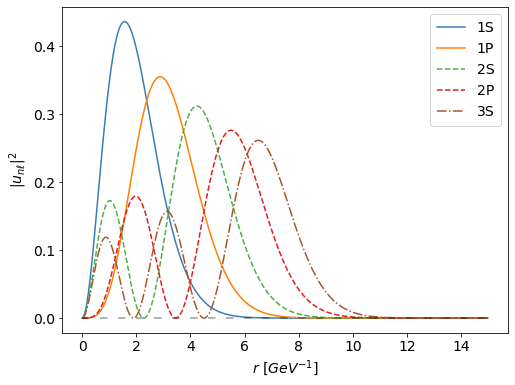
\includegraphics[width=\linewidth]{CornellSpectraLong.png}
    \caption{$|u_{n\ell}|^2$ of the states 1S,1P,2S,2P, and 3S found by the step method using the Cornell potential model, using $\beta_C \simeq 0.213$}
    \label{fig:CornellSpectra}
\end{figure}

\begin{figure}[!t]
    \centering
    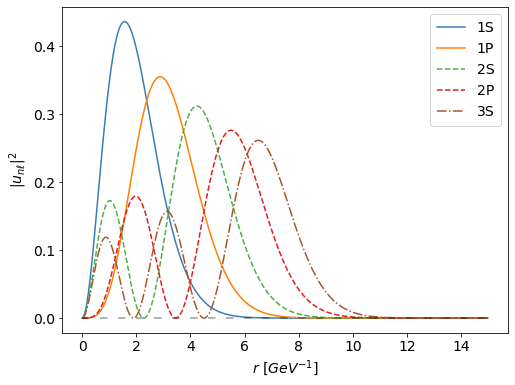
\includegraphics[width=\linewidth]{BhRuSpectraLong.png}
    \caption{$|u_{n\ell}|^2$ of the states 1S,1P,2S,2P, and 3S found by the step method using the Bhanot-Rudaz potential model, using $\beta_{BR} \simeq 0.206$}
    \label{fig:BhRuSpectra}
\end{figure}

\begin{figure}[!h]
    \centering
    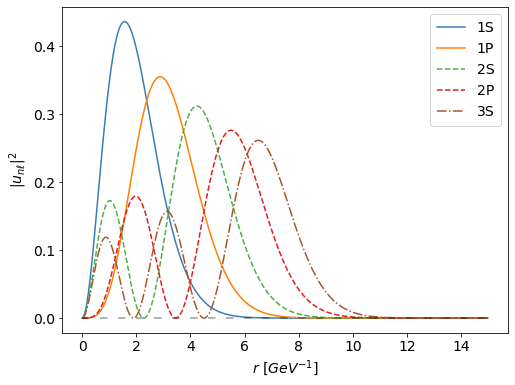
\includegraphics[width=\linewidth]{RichSpectraLong.png}
    \caption{$|u_{n\ell}|^2$ of the states 1S,1P,2S,2P, and 3S found by the step method using the Richardson potential model, using $\beta_R \simeq 0.410$}
    \label{fig:RichSpectra}
\end{figure}

\begin{figure}[!h]
    \centering
    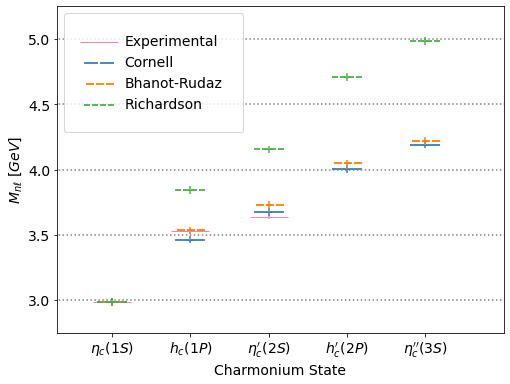
\includegraphics[width=\linewidth]{MassLines.png}
    \caption{A Mass line spectra of the $\eta_c(1S)$,$h_c(1P)$,$\eta_c'(2S)$,$h_c'(2P)$,$\eta_c''(3S)$ states in $GeV$, with error bars.}
    \label{fig:MassLines}
\end{figure}

\section{Discussion} 

Firstly, the results for $M_{h_c'}$ and $M_{\eta_c''}$ seem to be good predictions, though will possibly be slightly to high. The wavefunctions are all well behaved with $u_{n\ell}\rightarrow 0$ for $r\rightarrow \infty$ as desired; the $M_{\eta_c}$ predictions have a relative difference of no more than $8.7\times10^{-13}\%$ showing good calibration of the model parameters; and the Cornell and Bhanot-Rudaz predictions has relative differences of $1.81\%$ and $0.23\%$ with $M_{h_c}$, and also $1.02\%$ and $2.45\%$ with $M_{\eta_c'}$.However there are two notes. First, both the Cornell and Bhanot-Rudaz models make slight over predictions for $M_{\eta_c'}$ state, which may continue to higher masses. Second, the gap between an eigenvalue and the next should decrease for higher states, but the difference between $M_{h_c}$ and $M_{\eta_c'}$ for both Cornell and Bhanot-Rudaz is $\sim 0.2GeV$ but between $M_{\eta_c'}$ and $M_{h_c'}$ is $\sim 0.3GeV$. So therefore, it is not unreasonable to believe the masses found here are slightly over the actual mass of the charmonium states, and may act as an upper bound for experimental investigations.



It can be seen that in these findings the Richardson potential model\textbf{Eq.\ref{eqn:RichV}}, had the least agreement with experimental results, only growing at higher states. This can be seen in Fig.\ref{fig:MassLines} as the gap between the experimental and Richardson masses grows larger for each state. This must be from the $1/r$ term as the $r$ term is the same as the Cornell model, which has good agreement. There can be many reasons for this, ranging in complexity.
First, the issue may simply be that the approximation of two leading terms is not accurate enough for accurate predictions, in which case further works would need to more fully use the Fourier transform in calculations using this potential. Second, this work does not consider perturbation effects, but the additional detail of the coefficient of the $1/r$ term is meant to account for these. There for this perturbation correction is likely what leads to the over prediction of the energy, and so mass, of the charmonia, as it will introduce energetic effects this work does not account for in calculation.


The Bhanot-Rudaz prediction starts in good agreement up to $M_{h_c}$, then at $M_{\eta_c'}$ its predictions grow larger then the Cornell prediction. The 2S state peak is after $r > r_2$ where the Bhanot-Rudaz enters it's long-range regime. This implies the long-range regime returns potentials too high despite similarity the Cornell model's behaviour at this range, a linear confining potential. This would suggest that the coulombic one-gluon term is still not negligible at this range, despite the linear term being dominant, as it would serve to reduce the potential which has been shown necessary for higher accuracy. The implication of this is that the one-gluon interactions that the coulombic part represents still occur out to $r=15GeV^{-1}$. 
One note however is the more accurate prediction of $M_{1P}$. The 1P peak is in the mid-range regime of the Bhanot-Rudaz potential, which may suggest the logarithmic part is a more accurate representation of the quark-antiquark potential in this range. This may show a model more closely motivated by QCD can make more accurate predictions for lower energy states. This may infer that when the quarks are closer and the finer details are not being dominated by a large binding energy, and must be considered.

Unlike the Richardson and Bhanot-Rudaz model, the Cornell model does not have a term to account for spin. This simplification lends more agreement in these findings as spin has been ignored in calculation, and only singles states with unaligned spins have been considered. So, it seems the Cornell model is best fit as it neglects the same factors as this work. 
The Cornell potential was deemed to be the most suitable potential for prediction of higher state masses due to it's good predictions for the 1P and 2S masses, and agreeing with the 2S mass more so than the Bhanot-Rudaz predictions. 


\section{Conclusions}
 
 It is possible to find, accurately, the masses of charm-anticharm states using a numerical solving of the Schr\"odinger equation.
The wavefunction of the Schr\"odinger equation can be made into two coupled ODEs in terms of $\ell$, $V(r)$, and $E_{n\ell}$, where $V(r)$ is the potential model of Cornell \cite{CornellPaper}, Bhanot and Rudaz \cite{BhRoPaper}, or Richardson \cite{RichardsonPaper} here. 
By gradually increasing the value of the parameter from $0$ in steps, while maintaining $E_{n\ell}$ at the correct experimental value, for the 1S state until the wavefunction obeys certain conditions, the parameters can be calibrated to predict the binding energy of higher states via this same stepping method. Then the mass of that state can be found as the $E_{n\ell} + 2m_c$. Once the masses for all the states with experimental values have been calculated, agreement can be tested to ascertain the methods validity to predict unmeasured states.

Here, the Cornell potential model had good agreement for all experimental values, having relative diffreences no more than $1.82\%$, so was used to predict masses of the unstable $h_c'(2P)$ and $\eta_c(3P)$ states, which were found to be $M_{h_c'} = 4.003 \pm 0.03 GeV$, and $M_{\eta_c''} = 4.190 \pm  0.03 GeV$, though this maybe a slight over estimation.

Overall, it can be seen via the good agreement with experimental masses that this simplistic approach to calculating masses, paired with a simplistic potential model only describing the short and long range quark interactions, can still make good predictions on the masses of as of yet undiscovered states of charmonia. Further validation of this could be found via analysis of bottomonium, as it has more states with experimental results from 1S to 4S and 1P to 3P\textbf{\cite{pdg}}. Further to this, an analysis of the $B_c$ meson ($c\overline{b}$ and/or $b\overline{c}$) would be a wide area of investigation as there are as yet only two states known states which themselves have unknown properties. 

Other future explorations from this could of course include the calculation of masses of even higher states of charmonium ($n>2$, $\ell > 2$ etc.), as well as a review into the efficacy for this step method in solving fine-split masses when spin is factored into calculation. Here only singlet states have been considered and spin effects neglected, however a review of splin-split behaviour would give insight into the effects spin has in chromodynamical systems.

\section{Multi-parameter Potential}\label{sec:Multi-parameterPotential}

So far the Martin potential model described in  \textbf{Eq.\ref{eqn:MartinV}} has been undiscussed. This is due to it's factors causing trouble in numerical solving. 
Firstly, due to having two parameters, the standard stepping method described in \textbf{Sec.\ref{sec:numericalSolution}} is not possible because the values of $A$ and $B$ will be both effect the potential simultaneously, so must be found simultaneously.

This is done computationally via creating two lists, $L_A$ and $L_B$, of values for $A$ and $B$, in steps $\Delta_A$ and $\Delta_B$. Then \textbf{Eq.\ref{eqn:coupledODEs}} is solved for each $A$ value in $L_A$ paired with each $B$ in $L_B$. Then the best solution is where the tail of the solution $u_{n\ell}$ is closest to $0$ and has the smallest slope $du_{n\ell}/dr$.
Values of $u_{10}(15GeV^{-1})$, which will be referred to as the tip, for each $A \in [0,2]$ and $B \in [0,2]$ pair can be seen in \textbf{Fig.\ref{fig:martinHeatmap}}, where the step size of each $\Delta_A = \Delta_B = \Delta_{A,B} \simeq 0.01$.

\begin{figure}[t]
    \centering
    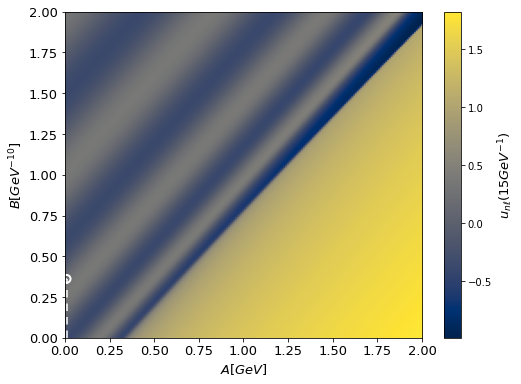
\includegraphics[width=\linewidth]{MartinHeatmap.png}
    \caption{A heatmap showing $u_{10}(15GeV^{-1}$ using the martin potential with $A,B \in [0,2]$}
    \label{fig:martinHeatmap}
\end{figure}

\begin{figure}[t]
    \centering
    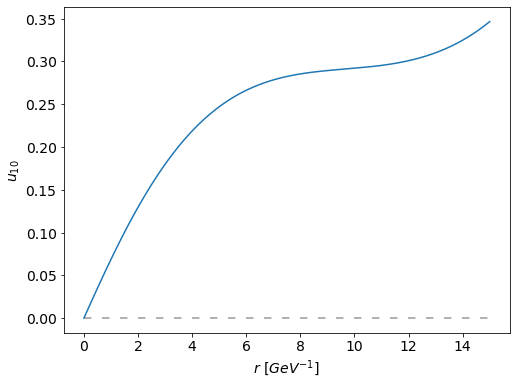
\includegraphics[width=\linewidth]{MartinBetaSpectra.png}
    \caption{$u_{10}$ bt $r$ with a Marting potential with $A \approx 0.01$ and $B \approx 0.36$.}
    \label{fig:martinSpectra}
\end{figure}

Firstly, there are noticeable diagonal blurred yellow regions running from low $A$ low $B$ to high $A$ high $B$, which represent areas of minimal tip value. 

In \textbf{\cite{MartinPaper}} $A_{ref}=8.064GeV, B_{ref}=6.8698GeV^{-10}$, but in these findings $A=0.01, B=0.36$ (both $\pm0.01$). Notably $A$ is a single step away from $0$, this implies the Martin potential shape and value are being decided entirely by the $B$ term, as $A$ is the smallest non-zero value numerically possible. Also, both $A$ and $B$ are far below the reference values, which causes inaccuracies in the solving of \textbf{Eq.\ref{eqn:coupledODEs}}. As can be seen in \textbf{Fig.\ref{fig:martinSpectra}}, the wavefunction starts to turn from its peak at $\sim 8GeV$, but instead of then going to $0$ the wavefunction inflects and starts going toward infinity.

One possible cause for this is the minimisation effect of the $\alpha = 0.1$ factor. $r \in [10^{-6}, 15]GeV^{-1}$ is the standard range that all other potentials have been solved over. However, the $0.1$ factor transfers this into $[0.251188643150958, 1.31101942303975]$ with $\Delta_r = 0.00013141077157907688$. Python uses the float type to store decimal numbers, which has an accuracy of approximately 7 decimal places, so python will be using $r \in [0.2511886, 1.3110194]$, with $\Delta_r = 0.0001314$. These small numbers that python is not well able to handle will then be causing numerical instability, which will cause more calculations to have a larger divergence. This means a method based on divergence minimisation will not be as able to find a solution as tips near $0$ will not occur. 

The other possibility is that $\Delta_{A,B}$ is too large to approach a solution. As can be seen from the shape of $u_{10}$ in \textbf{Fig.\ref{fig:martinSpectra}}, the solution almost starts to return to $0$, so is maybe near the solution but steps over it due to the step size. If the solution is being stepped over due to the step size then the program will not be able to find it. Unfortunately, making $\Delta_{A,B}$ smaller would have a compounding time scaling effect due to the $\mathcal{O}(n^2)$ of solving \textbf{Eq.\ref{eqn:coupledODEs}}. Overall then this issue of the step method minimising $A$ and the power of $0.1$ causing numerical instability leads to the Martin potential not being suitable in the prediction of masses of charmonia with the implementation in this work.
So then, in future work a more accurate and faster language (c++, Rust, etc.) may allow for better use of the Martin potential.



\printbibliography


\newpage

\section*{Error Appendix}
[The equations and methods used in this appendix are based on the error analysis formulae given in I.G. Hughes and T.P.A. Hase, \textit{Measurements and their Uncertainties}, Oxford university Press, Oxford (2010).]\newline

The error in the experimental masses and mass of quarks are given by particle data group \textbf{\cite{pdg}}: $\alpha_{m_c} = \pm0.02GeV$, $\alpha_{m_b} = ^{+0.03}_{-0.02}$, $\alpha_{M_{\eta_c}} = \pm0.4$, $\alpha_{M_{h_c}} = \pm0.11$, $\alpha_{M_{\eta_c'}} = \pm1.1$.

The resolution of the step method is the step size, so the error on the calibrated parameters is $\alpha_\beta = 9\times10^{-15}$ and for the binding energy eigenvalues will be, $\alpha_{E_{n\ell}} = 9\times10^{-15}$.

Similarly, $A$ and $B$ will have erros equal to the resolution of $L_A$ and $L_B$, so $\alpha_A = \alpha_B = 0.01$.

The mass of quarkonia is the sum of its binding energy eigenvalue and the mass of the constituent quarks, so the error will be,
\begin{equation*}
    \alpha_{M_{n\ell}} = \sqrt{(\alpha_{E_{n\ell}})^2 + (\alpha_{m_q})^2 + (\alpha_{m_\overline{q}}})^2.
\end{equation*}




\clearpage

\onecolumngrid %Puts Summary into single column

\section*{Scientific Summary for a General Audience}
\newline
\newline
Mesons are very small particles made of even smaller particles called quarks. Mesons made of heavier quarks are called quarkonium. The quarks in quarkonium are held together by a binding energy, which due to Einstein's $E=mc^2$ becomes part of the mass of the particle just as much as the mass of the quarks that make it.  Using Schr\"odinger's equation split into 2 linked equations, a computer program is able to find this binding energy, and so the mass of the quarkonium. The same quarkonium can be different in a quantum way, some being more energetic than others. So by testing if a computer can get close to the real masses of known quarkonium, the mass of as yet unmeasured quarkonia can be found. 

\end{document}